% GENERAL PROBLEM STATEMENT
In order to demonstrate the optimal inference of individual parameters, we devise a simple example within the domain of structural engineering for which we conduct a simulated computer experiment.
It should be understood as a benchmark of optimal combination of information in data analysis of engineering systems.
% EXPERIMENTAL SITUATION
An experimental situation is investigated where data are collected for an ensemble of identically manufactured beams.
The acquired specimen-specific data are informative to variable degree.
Therefore the goal is to optimally exploit the available information in the individual assessment of ensemble members that are poorly supported by experimental evidence.
\par % PHYSICAL MODEL
The system under consideration is a set of simply supported beams \(i=1,\ldots,n\) with well-known lengths \(L_i\), widths \(b_i\) and heights \(h_i\).
Beams are composed out of a material which is subject to aleatory uncertainty in its material properties, say the Young's modulus \(E_i\). 
For each individual beam \(i\) the elastic modulus \(E_i\) is assumed to be constant along its main axis.
Across the sample of beams Young's moduli \(E_i\) are distributed according to a lognormal distribution \(\mathcal{LN}(E_i \cond \mu_E,\sigma_E^2)\)
with mean value \(\mu_E = \mathds{E}[E_i]\) and variance \(\sigma_E^2 = \mathrm{Var}[E_i]\).
At positions \(s_j\) with \(j=1,\ldots,n_i\) and \(0 \leq s_j \leq L_i/2\) the deflections \(v_i(s_j)\) of the beams under concentrated point loads \(F_i\) at midspan are calculated as
\begin{equation} \label{eq:ForwardModel}
  v_i(s_j) = \frac{F_i s_j }{48 E_i I_i} \left( 3 L_i^2 - 4s_j^2 \right).
\end{equation}
Here the moment of inertia is given as \(I_i = b_i h_i^3 / 12\).
A symmetric expression holds for positions \(s_j\) with \(L_i/2 \leq s_j \leq L_i\).
% VISUALIZATION
In \cref{fig:Beam} a sketch of a simply supported beam is drawn.
% INVERSE PROBLEMS
In a series of experiments measured beam deflections can be used to estimate individual realizations \(E_i\) or the hyperparameters \((\mu_E,\sigma_E)\).
Herein we consider the inference of the Young's modulus \(E_{\analyzed}\) of a beam \(\analyzed \in \{1,\ldots,n\}\) for which it is assumed that experimental evidence is scarce.
A simulated computer experiment is conducted as described below.
\begin{figure}[ht]
  \centering
  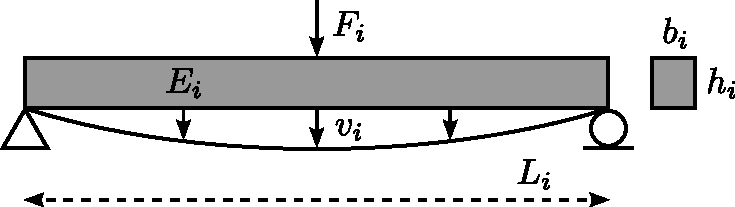
\includegraphics[width=\JRUESbeamWidth]{fig_JRUES_Beam}
  \caption[Simply supported beam]{Simply supported beam.}
  \label{fig:Beam}
\end{figure}
\par % INVERSE PROBLEM
We choose a set of \(n=100\) beams with well-known and constant dimensions \(L_i=\unit[1]{m}\) and \(b_i=h_i=\unit[10]{cm}\) that are subjected to loads \(F_i=\unit[30]{kN}\).
The elastic moduli \(E_i\) are randomly sampled from a lognormal distribution with mean \(\mu_E=\unit[15]{GPa}\) and standard deviation \(\sigma_E=\unit[3]{GPa}\).
% PSEUDO-DATA
We simulate a synthetic set of pseudo-data \(\bm{y}_{i}=(y_{i1},y_{i2},y_{i3})\) for each beam.
For \(j=1,2,3\) pseudo-observations \(y_{ij}=v_i(s_j)+\epsilon_{ij}\) are generated for positions \(\bm{s}_i = (s_1,s_2,s_3)\)
with \(s_1=\unit[25]{cm}\), \(s_2=\unit[50]{cm}\) and \(s_3=\unit[75]{cm}\) by perturbing the corresponding model predictions \cref{eq:ForwardModel}.
The residuals \(\bm{\varepsilon}_i = (\varepsilon_{i1},\varepsilon_{i2},\varepsilon_{i3})\) are independently sampled from centered Gaussians
\(\mathcal{N}(\bm{\varepsilon}_i \cond \bm{0},\bm{\Sigma}_i)\) with covariance matrices \(\bm{\Sigma}_i = \operatorname{diag}(\sigma_{i1}^2,\sigma_{i2}^2,\sigma_{i3}^2)\).
We choose comparably small residual standard deviations \(\sigma_{ij} = \unit[0.01]{cm}\) for \(i \neq \analyzed\) and comparably large deviations \(\sigma_{\analyzed j} = \unit[0.1]{cm}\).
% INTERPRETATION
This represents an experimental situation where the ensemble of beams is tested, however, the data are less informative about the specimen \(\analyzed\).
\par % HYPERPRIOR
We assume that the hyperparameter values \((\mu_E,\sigma_E)\) are not known, yet prior or expert knowledge is available.
The inferential prior of the hyperparameters is set as the independent distribution \(\pi(\mu_E,\sigma_E) = \pi(\mu_E) \, \pi(\sigma_E)\)
with weakly informative but proper uniform distributions \(\pi(\mu_E)=\mathcal{U}(\mu_E \cond 0,100)\) and \(\pi(\sigma_E) \sim \mathcal{U}(\sigma_E \cond 0,30)\) (in \(\unit[]{GPa}\)) as marginals.
% INTERPRETATION
This represents the scenario that the available prior knowledge does not allow to assign more informative priors.
Nonetheless the hyperparameter values are physically bounded by zero from below and they can be priorly bounded from above.
Thus values that are outside of the specified interval can be excluded.
\par % PROBLEM STATEMENT
In the following we conduct inference of the Young's modulus \(E_{\analyzed}\) of a beam \(\analyzed\).
% UNKNOWNS
The hyperparameter values \((\mu_E,\sigma_E)\) and the randomly sampled elastic moduli \(\tuple{E_i}\) are treated as ``unknowns''.
% TRUE VALUE
This includes the ``true'' parameter value \(E_{\analyzed} = \unit[17.01]{GPa}\).
% KNOWNS
The measurement locations \(\tuple{\bm{s}_i}\), applied loads \(\tuple{F_i}\) and physical beam dimensions \(\tuple{L_i,b_i,h_i}\) are the well-known experimental conditions.
Further knowns comprise the parametric prior \(\pi(\mu_E,\sigma_E)\), the levels of measurement uncertainty \(\tuple{\bm{\Sigma}_i}\) and the data \(\tuple{\bm{y}_i}\).
% THREE APPROACHES
The described experimental setup is studied next.
Simple Bayesian updating, staged estimation and multilevel inversion are demonstrated.
The flow of information is investigated and insight into the inferential mechanism is provided.
% MCMC
Low-dimensional posteriors are generally computed by means of a RWM algorithm, while higher-dimensional posteriors are computed by means of HMC/RWM hybrid sampler.
The latter is based on updating the parameters via Hamiltonian dynamics while updating the hyperparameters with a random walk.
% ALGORITHMIC EFFICIENCY
Finally the implementation of the samplers is described in detail.
Furthermore, the efficiency of HMC/RWM sampling is contrasted with pure RWM sampling.

\subsection{Simple updating}
% COMPOUND PRIOR
The compound prior \cref{eq:MixturePrior} may not be available in analytical form, however, one can sample the prior by the method of composition \cite{MCMC:Zio2013}.
To that end one draws \(K\) samples from the hyperparameter distribution \(\pi(\mu_E,\sigma_E)\).
Subsequently one draws a sample from the parameter distribution \(\mathcal{LN}(E_i \cond \mu_E,\sigma_E^2)\) for each hyperparameter realization.
As desired the sample of parameter values is distributed according to the mixture in \cref{eq:MixturePrior}.
We draw \(K = 10^5\) random samples of the mixture prior.
In \cref{fig:MixturePrior} a kernel density estimate of the mixture is shown.
It is seen that the mixture is approximated well by kernel smoothing.
In the following MCMC analysis the prior of \(E_{\analyzed}\) is therefore represented as the obtained kernel density estimate.
% POSTERIOR SAMPLING
We accomplish Bayesian updating by sampling the one-dimensional posterior \(\pi(E_{\analyzed} \cond \bm{y}_{\analyzed})\) with a simple RWM sampler.
In \cref{fig:SimpleInversion} the simulated posterior is shown.
% EXPERIMENTAL RESULTS
The posterior of \(E_{\analyzed}\) has the mean \(\mu_{E_{\analyzed}} = \unit[21.73]{GPa}\) and the standard deviation \(\sigma_{E_{\analyzed}} = \unit[5.49]{GPa}\).
With a coefficient of variation \(\mathrm{CV} = \unit[25]{\%}\) this corresponds to a relatively high degree of posterior uncertainty.
The maximum a posteriori (MAP) estimate of the modulus \(E_{\analyzed}\), i.e.\ the posterior mode, is found to be \(\hat{E}_{\analyzed}^{\mathrm{MAP}} = \unit[19.07]{GPa}\).
Compared to the true value \(E_{\analyzed} = \unit[17.01]{GPa}\) the relative approximation error of the MAP estimate is \(\epsilon = \unit[12]{\%}\).
% FIGURES: SIMPLE UPDATING
\begin{figure}[ht]
  \begin{minipage}[b]{0.49\linewidth}
    \centering
    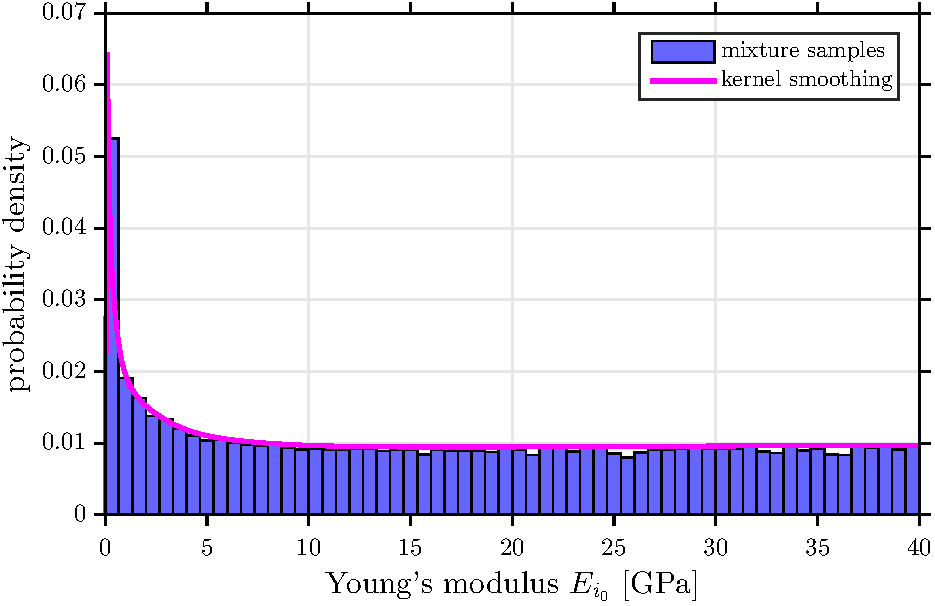
\includegraphics[width=\JRUESfigWidth]{fig_JRUES_UpdatingPrior}
    \caption[Simple updating: prior]{Simple updating: prior.}
    \label{fig:MixturePrior}
  \end{minipage}%
  \hfill
  \begin{minipage}[b]{0.49\linewidth}
    \centering
    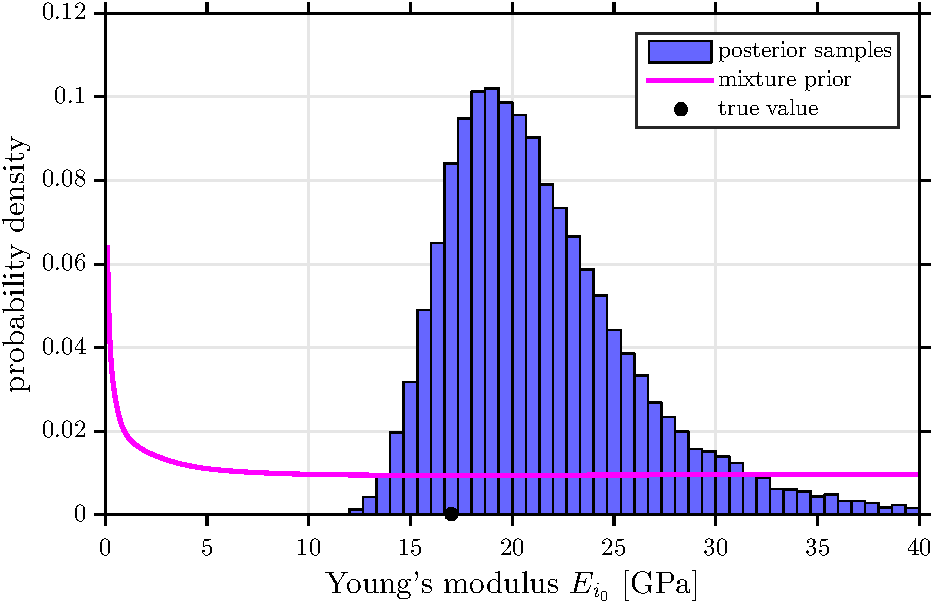
\includegraphics[width=\JRUESfigWidth]{fig_JRUES_UpdatingPosterior}
    \caption[Simple updating: posterior]{Simple updating: posterior.}
    \label{fig:SimpleInversion}
  \end{minipage}%
\end{figure}

\subsection{Staged estimation}
% PROBABILISTIC INVERSION
First we conduct probabilistic inversion to infer the hyperparameters \((\mu_E,\sigma_E)\) with data \(\tuple{\bm{y}_{\notanalyzed}}\).
% MULTILEVEL INVERSION & HMC
The high-dimensional posterior \(\pi(\tuple{E_{\notanalyzed}},\mu_E,\sigma_E \cond \tuple{\bm{y}_{\notanalyzed}})\) is therefore computed via HMC sampling.
The implementation of the sampler is described later on.
For the time being we remark that \(N=10^6\) posterior samples are drawn within a runtime of ca.\ \(t = \unit[1]{h}\).
% NEW MIXTURE PRIOR
A thinned sample of the posterior \(\pi(\mu_E,\sigma_E \cond \tuple{\bm{y}_{\notanalyzed}})\) is used to draw \(K=10^5\) samples from \cref{eq:Filtering:Prior} by the composition method.
The resulting sample from \(\pi(E_{\analyzed} \cond \tuple{\bm{y}_{\notanalyzed}})\) is shown in \cref{fig:NewMixturePrior} along with a lognormal fit to the sample.
Since the lognormal fit reproduces the desired distribution adequately well, it is utilized as the prior \(\pi(E_{\analyzed} \cond \tuple{\bm{y}_{\notanalyzed}})\) in the subsequent updating step.
% SUBSEQUENT UPDATING
The resulting univariate posterior \(\pi(E_{\analyzed} \cond \tuple{\bm{y}_{\notanalyzed}},\bm{y}_{\analyzed})\) is shown in \cref{fig:SubsequentInversion}.
% EXPERIMENTAL RESULTS
The final posterior of \(E_{\analyzed}\) has the mean \(\mu_{E_{\analyzed}} = \unit[17.44]{GPa}\) and the standard deviation \(\sigma_{E_{\analyzed}} = \unit[2.17]{GPa}\).
With \(\mathrm{CV} = \unit[12]{\%}\) the posterior features a lower degree of uncertainty as compared to simple updating.
Likewise the relative error \(\epsilon = \unit[1]{\%}\) of the MAP estimate \(\hat{E}_{\analyzed}^{\mathrm{MAP}} = \unit[16.84]{GPa}\) is much smaller.
% FIGURES: BAYESIAN FILTERING
\begin{figure}[ht]
  \begin{minipage}[b]{0.49\linewidth}
    \centering
    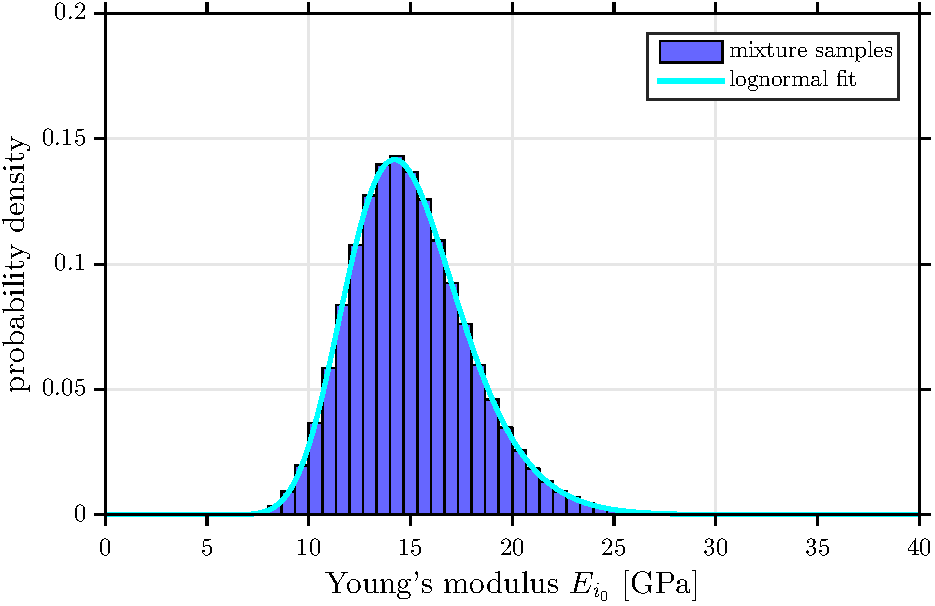
\includegraphics[width=\JRUESfigWidth]{fig_JRUES_FilteringPrior}
    \caption[Staged estimation: prior]{Staged estimation: prior.}
    \label{fig:NewMixturePrior}
  \end{minipage}%
  \hfill
  \begin{minipage}[b]{0.49\linewidth}
    \centering
    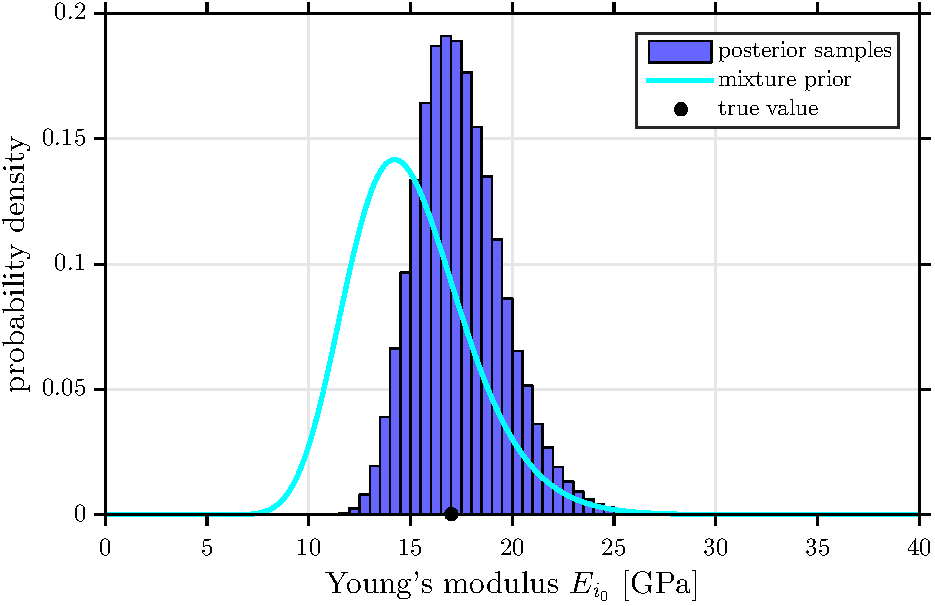
\includegraphics[width=\JRUESfigWidth]{fig_JRUES_FilteringPosterior}
    \caption[Staged estimation: posterior]{Staged estimation: posterior.}
    \label{fig:SubsequentInversion}
  \end{minipage}%
\end{figure}
\par % DISCUSSION
Summarized, the posterior \(\pi(E_{\analyzed} \cond \tuple{\bm{y}_{\notanalyzed}},\bm{y}_{\analyzed})\) shown in \cref{fig:SubsequentInversion}
is a better representation of the true value than \(\pi(E_{\analyzed} \cond \bm{y}_{\analyzed})\) depicted in \cref{fig:SimpleInversion}.
The reason is that the prior \(\pi(E_{\analyzed} \cond \tuple{\bm{y}_{\notanalyzed}})\) plotted in \cref{fig:NewMixturePrior}
contains more information than \(\pi(E_{\analyzed})\) shown in \cref{fig:MixturePrior}.
This illustrates the flow of information from data \(\tuple{\bm{y}_{\notanalyzed}}\) towards \(E_{\analyzed}\) that was already discussed.
The information exchange takes place in an indirect way.
While staged estimation requires the consecutive solution of two different problems, i.e.\ probabilistic inversion and subsequent updating,
multilevel inversion is more elegant and satisfactory in the sense that it allows to consistently perform those two separate tasks at once.
This is demonstrated next.

\subsection{Multilevel inversion}
% JOINT POSTERIOR
Full multilevel inversion is finally performed by sampling the joint posterior \(\pi(\tuple{E_i},\mu_E,\sigma_E \cond \tuple{\bm{y}_i})\).
The employed MCMC sampler is described and benchmarked afterwards.
Samples from the marginal \cref{eq:Multilevel:MarginalPosterior} can easily be extracted by discarding samples from \(\tuple{E_{\notanalyzed}}\) and \((\mu_E,\sigma_E)\).
The marginal posterior \(\pi(E_{\analyzed} \cond \tuple{\bm{y}_i})\) is plotted in \cref{fig:JointInversion}.
% EXPERIMENTAL RESULTS
It has the mean \(\mu_{E_{\analyzed}} = \unit[17.44]{GPa}\) and the standard deviation \(\sigma_{E_{\analyzed}} = \unit[2.18]{GPa}\) which rounds up to \(\mathrm{CV} = \unit[13]{\%}\).
The relative error of the MAP estimate \(\hat{E}_{\analyzed}^{\mathrm{MAP}} = \unit[16.86]{GPa}\) is \(\epsilon = \unit[1]{\%}\).
% SUMMARY
As a summary the simulated posteriors \(\pi(E_{\analyzed} \cond \bm{y}_{\analyzed})\), \(\pi(E_{\analyzed} \cond \tuple{\bm{y}_{\notanalyzed}},\bm{y}_{\analyzed})\)
and \(\pi(E_{\analyzed} \cond \tuple{\bm{y}_i})\) that are relevant to the identification of \(E_{\analyzed}\) are shown in \cref{fig:PosteriorSummary}.
The corresponding means, modes and standard deviations (SD) are listed in \cref{tab:PosteriorSummary}.
% FIGURES: MULTILEVEL INVERSION & SUMMARY
\begin{figure}[ht]
  \begin{minipage}[b]{0.49\linewidth}
    \centering
    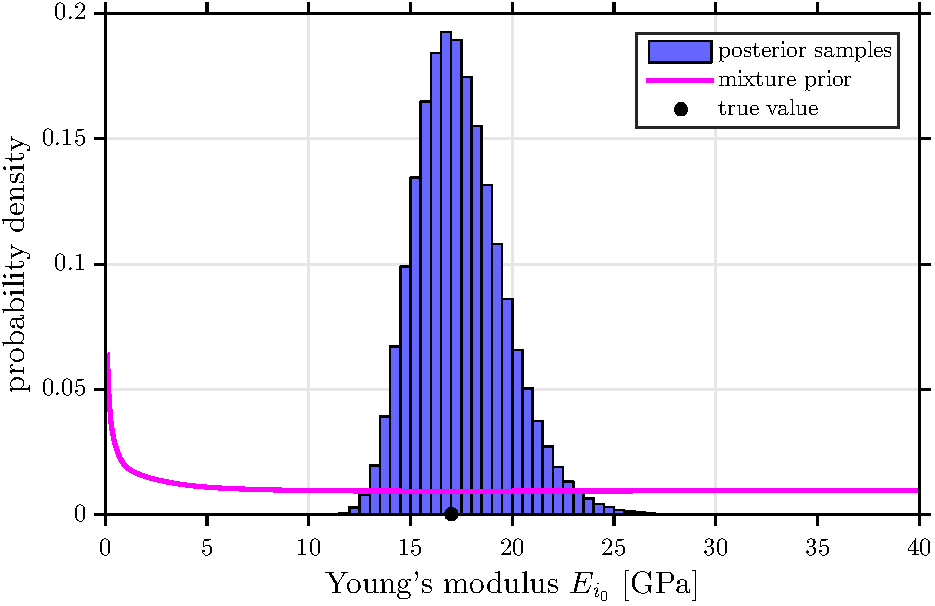
\includegraphics[width=\JRUESfigWidth]{fig_JRUES_JointPosterior}
    \caption[Multilevel inversion: posterior]{Multilevel inversion: posterior.}
    \label{fig:JointInversion}
  \end{minipage}%
  \hfill
  \begin{minipage}[b]{0.49\linewidth}
    \centering
    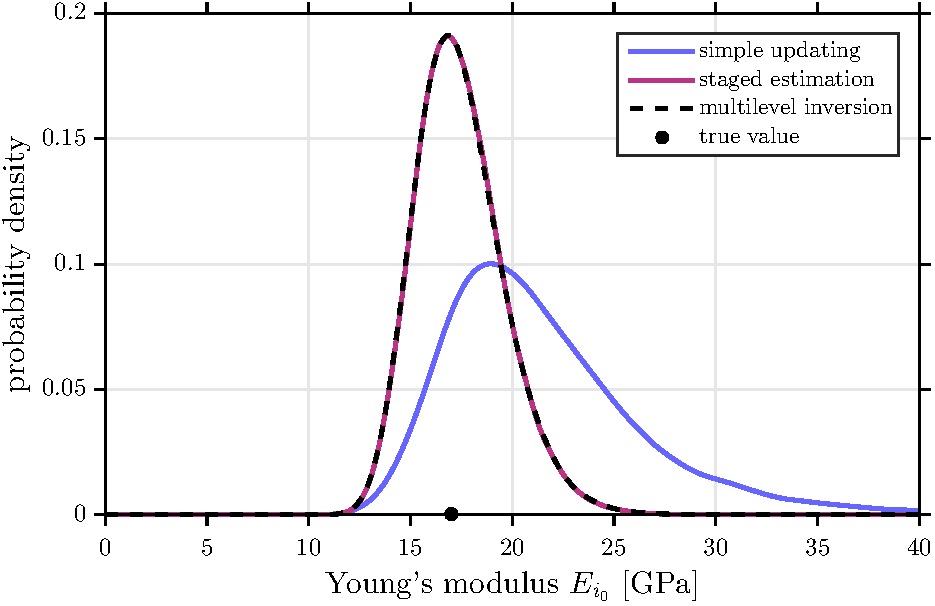
\includegraphics[width=\JRUESfigWidth]{fig_JRUES_PosteriorSummary}
    \caption[Summary of the posteriors]{Summary of the posteriors.}
    \label{fig:PosteriorSummary}
  \end{minipage}%
\end{figure}
% TABLE: SUMMARY
\begin{table}[htbp]
  \caption[Summary of estimating \(E_{\analyzed}\)]{Summary of estimating \(E_{\analyzed}\).}
  \label{tab:PosteriorSummary}
  \centering
  \begin{tabular}{rccc}
    \toprule
    Approach & Mean \(\lbrack\unit[]{GPa}\rbrack\) & Mode \(\lbrack\unit[]{GPa}\rbrack\) & SD \(\lbrack\unit[]{GPa}\rbrack\) \\
    \midrule
    Simple updating      & \(21.73\) & \(19.07\) & \(5.49\) \\
    Staged estimation    & \(17.44\) & \(16.84\) & \(2.17\) \\
    Multilevel inversion & \(17.44\) & \(16.86\) & \(2.18\) \\
    \bottomrule
  \end{tabular}
\end{table}
\par % DISCUSSION
As expected, the posterior \(\pi(E_{\analyzed} \cond \tuple{\bm{y}_i})\) shown in \cref{fig:JointInversion} is nearly identical to
\(\pi(E_{\analyzed} \cond \tuple{\bm{y}_{\notanalyzed}},\bm{y}_{\analyzed})\) in \cref{fig:SubsequentInversion}.
% SHRINKAGE & INFORMATION
By comparison with the corresponding posterior \(\pi(E_{\analyzed} \cond \bm{y}_{\analyzed})\) in \cref{fig:SimpleInversion},
the additional amount of information relating to \(E_{\analyzed}\) that has been gained by utilizing the full set of observations \(\tuple{\bm{y}_i}\) becomes apparent from the associated shrinkage of the posterior uncertainty.
% JOINT POSTERIOR
A manifest advantage of multilevel inversion over staged estimation is that it incidentally provides information about all unknowns \((\tuple{E_i},\mu_E,\sigma_E)\).
The posterior \(\pi(\tuple{E_i},\mu_E,\sigma_E \cond \tuple{\bm{y}_i})\) accumulates information such that the whole data \(\tuple{\bm{y}_i}\) contributes to the collective learning process.
This is advantageous in the case that not just a single realization \(E_{\analyzed}\) but a larger subset of \(\tuple{E_i}\) is of inferential interest.
% TIME DEPENDENCY
While staged estimation mainly served the purpose of illustrating the presence and manner of the abovementioned learning process,
it is practical in experimental situations where data are not collected at the same time.
In this case the sequential approach allows to analyze newly observed data without the need for resolving the full multilevel problem again.

\subsection{Algorithmic efficiency}
The efficacy and viability of HMC sampling for exploring multilevel posteriors is now investigated.
In the last two sections the algorithm was used to compute the posteriors
\(\pi(\tuple{E_{\notanalyzed}},\mu_E,\sigma_E \cond \tuple{\bm{y}_{\notanalyzed}})\) and \(\pi(\tuple{E_i},\mu_E,\sigma_E \cond \tuple{\bm{y}_i})\).
The latter involves a \(102\)-dimensional parameter space.
In order to assess the performance gain by HMC sampling the algorithm is compared to a classical RWM algorithm.
% RANDOM WALK METROPOLIS
The RMW sampler is implemented in a blocked manner where the block of hyperparameters and the one of the parameters are updated separately.
Gaussian proposal distributions with covariance matrices \(\bm{\Sigma}_{(\mu_E,\sigma_E)} = \operatorname{diag}(0.3,0.3)\) and \(\bm{\Sigma}_{\tuple{E_i}} = \operatorname{diag}(\sigma_1^2,\ldots,\sigma_n^2)\) are used.
The latter is defined by setting \(\sigma_{\analyzed} = 0.3\) and \(\sigma_i = 0.002\) for \(i \neq \analyzed\).
This takes the different scales of the posterior marginals into account.
% INITIALIZATION
The sampler is initialized at maximum likelihood estimates of individual parameters in separate deterministic inverse problems and two-stage estimates of the hyperparameters.
This procedure initializes the algorithm close to the posterior modes.
% RUNNING
The MCMC execution time to draw \(N = 10^7\) posterior samples amounts to ca.\ \(t = \unit[5]{h}\).
Acceptance rates of ca.\ \(\unit[22]{\%}\) for the parameters and ca.\ \(\unit[25]{\%}\) for the hyperparameters are noticed.
\par % HAMILTONIAN MONTE CARLO
The HMC/RWM sampler features the same blockwise updating structure.
Hyperparameters are updated by the same random walk updates that were described above.
The parameters are updated with HMC proposals.
% DERIVATIVES
For the present problem all necessary partial derivatives are analytically obtained.
% MASS MATRIX
A diagonal mass matrix \(\bm{M} = \operatorname{diag}(m_1,\ldots,m_n)\) is used.
The point masses are set to \(m_i = 20\) for \(i \neq \analyzed\) and to \(m_{\analyzed} = 0.15\) for the QoI.
This tuning accounts for the different marginal scales of the parameters.
More details about relative parameter scalings can be found in \cite{MCMC:Neal2011}.
% DYNAMICS
For the dynamical simulation the parameters are set as follows.
The number of leapfrog steps is set to \(L = 8\).
At the start of the trajectory the discretized stepsize \(\Delta\tau\) in fictional time is randomized within the interval \([0.15,0.16]\).
It is kept fixed throughout each dynamical simulation, though.
This avoids potentially occurring problems such as slow mixing or even of non-ergodicity due to (nearly) exact periodicity of the system trajectories \cite{MCMC:Mackenzie1989}.
The used parameter tuning leads to stable trajectories while it also ensures that long distances in the parameter space are traversed.
% INITIALIZATION
Initialization is accomplished as before.
% RUNNING
A number of \(N = 10^6\) MCMC iterations are executed within an execution runtime of ca.\ \(t = \unit[1]{h}\).
The dynamical HMC parameter updates are accepted with a rate of ca.\ \(\unit[100]{\%}\).
In the hyperparameter block the acceptance rate is ca.\ \(\unit[25]{\%}\).
\par % TRACE PLOTS
The Markov chains produced by the RWM and the HMC sampler are compared with each other.
In \cref{fig:Trace:RWM,fig:Trace:HMC} the converged chains for \(E_{\analyzed}\) are shown for \(5000\) MCMC iterations.
These trace plots show how the chains sample the corresponding posterior marginals around their means.
Obviously the mixing properties of the HMC chain are better than the ones of the RWM chain.
% AUTOCORRELATION
The sample autocorrelation function (ACF) gives greater insight into the characteristics of the samplers.
In \cref{fig:ACF:RWM0,fig:ACF:HMC0} the ACFs of the two chains are shown for the QoI \(E_{\analyzed}\).
It can be seen that for RWM sampling the ACF drops to zero within ca.\ \(1000\) MCMC iterations.
In contrast the ACF of the HMC chain dies down within ca.\ five iterations.
% FIGURES: TRACE PLOTS
\begin{figure}[ht]
  \begin{minipage}[b]{0.49\linewidth}
    \centering
    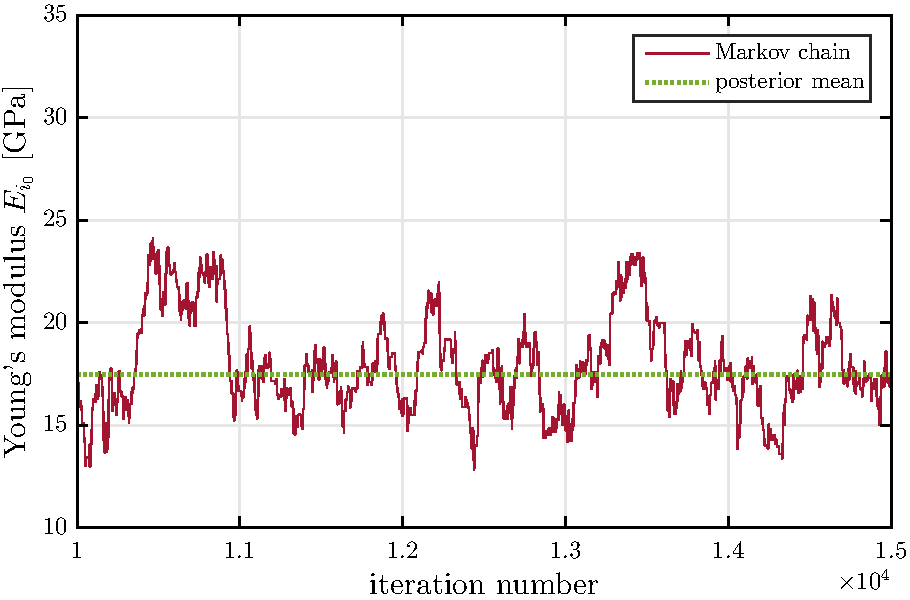
\includegraphics[width=\JRUESfigWidth]{fig_JRUES_Trace_RWM0}
    \caption[RWM: Trace plot of \(E_{\analyzed}\)]{RWM: Trace plot of \(E_{\analyzed}\).}
    \label{fig:Trace:RWM}
  \end{minipage}%
  \hfill
  \begin{minipage}[b]{0.49\linewidth}
    \centering
    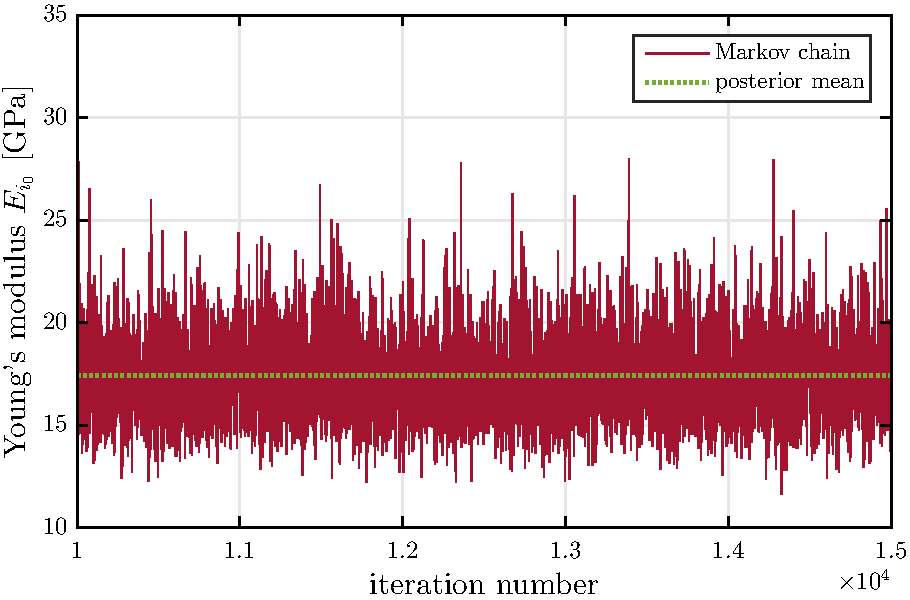
\includegraphics[width=\JRUESfigWidth]{fig_JRUES_Trace_HMC0}
    \caption[HMC: Trace plot of \(E_{\analyzed}\)]{HMC: Trace plot of \(E_{\analyzed}\).}
    \label{fig:Trace:HMC}
  \end{minipage}%
\end{figure}
% FIGURES: ACF
\begin{figure}[ht]
  \begin{minipage}[b]{0.49\linewidth}
    \centering
    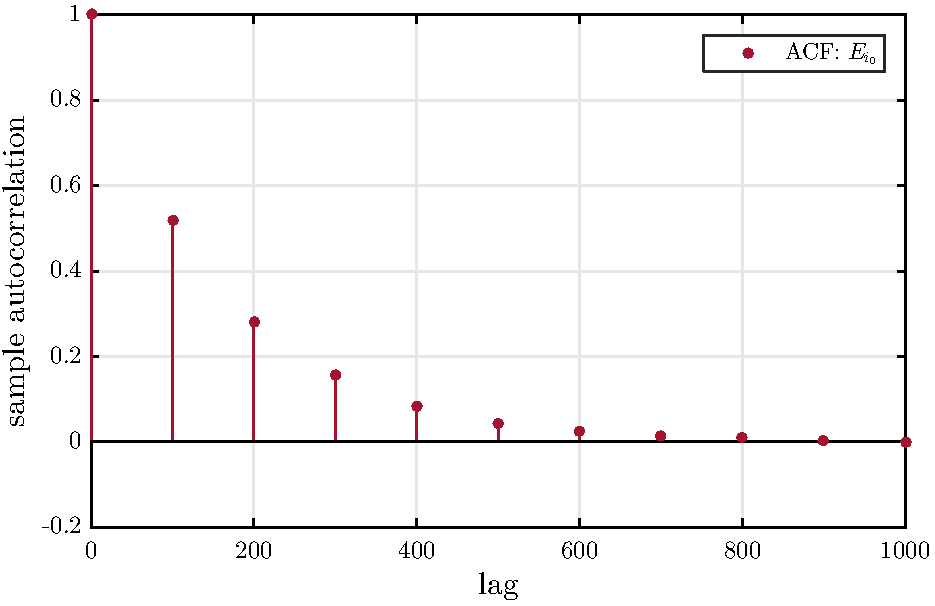
\includegraphics[width=\JRUESfigWidth]{fig_JRUES_ACF_RWM0}
    \caption[RWM: ACF of \(E_{\analyzed}\)]{RWM: ACF of \(E_{\analyzed}\).}
    \label{fig:ACF:RWM0}
  \end{minipage}%
  \hfill
  \begin{minipage}[b]{0.49\linewidth}
    \centering
    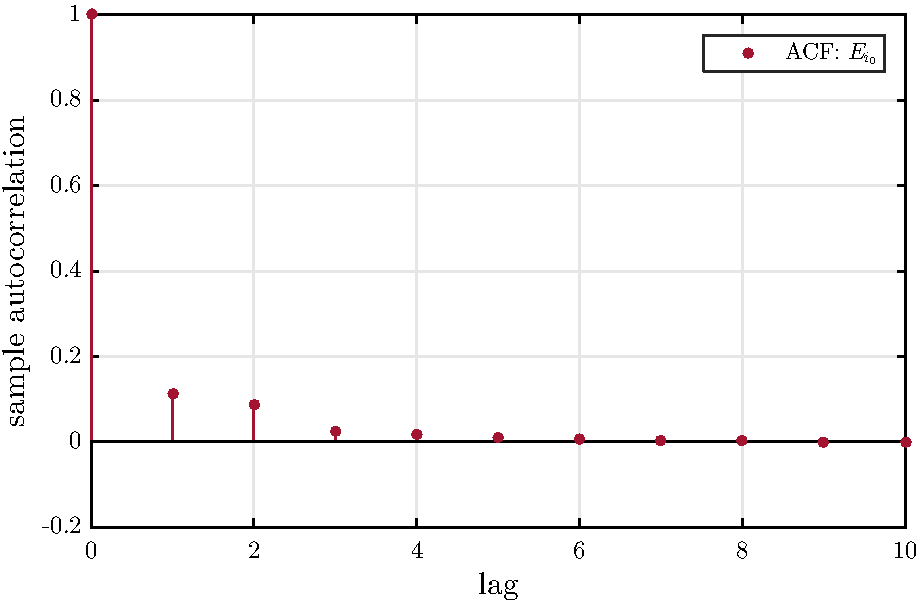
\includegraphics[width=\JRUESfigWidth]{fig_JRUES_ACF_HMC0}
    \caption[HMC: ACF of \(E_{\analyzed}\)]{HMC: ACF of \(E_{\analyzed}\).}
    \label{fig:ACF:HMC0}
  \end{minipage}%
\end{figure}
\par % EFFECTIVE SAMPLE SIZE
With the ACF one can approximately assess the effective sample size \(N_{\mathrm{eff}}\) in \cref{eq:MCMC:EstimationVariance}.
A variety of methods for assessing the estimation variance \(\sigma^2_{\bar{E}_{\analyzed}} = N^{-1} \sigma^2_{E_{\analyzed}} \tau_{\mathrm{int}}\)
and the effective sample size \(N_{\mathrm{eff}} = N / \tau_{\mathrm{int}}\) have been proposed \cite{MCMC:Flegal2008,MCMC:Flegal2010}.
The simplest method rests upon the substitution of \(\sigma^2_{E_{\analyzed}}\) and \(\tau_{\mathrm{int}}\) by estimators \cite{MCMC:Ripley1987,MCMC:Kass1998}.
% APPROXIMATION
We use a sample estimate \(\hat{\sigma}^2_{E_{\analyzed}}\) and a truncated series approximation \(\hat{\tau}_{\mathrm{int}} = 1 + 2 \sum_{s=1}^r \hat{\rho}_s\).
The sum is cut off at the smallest lag \(r\) for which the absolute value of the empirical autocorrelation \(\hat{\rho}_r\) drops below a certain threshold \(\left| \hat{\rho}_r \right| < 0.01\).
% RESULTS
For the RWM chain with a total number of iterations \(N=10^7\) that were done in \(t = \unit[5]{h}\) one obtains an effective sample size \(N_{\mathrm{eff}} = 3 \cdot 10^4\)
and a Monte Carlo standard error (MCSE) \(\sigma_{\bar{E}_{\analyzed}} = \unit[1.5 \cdot 10^{-2}]{GPa}\) for estimating \(E_{\analyzed}\).
The effective sample size and the MCSE for the HMC chain with \(N=10^6\) and \(t = \unit[1]{h}\) equal to \(N_{\mathrm{eff}} = 7 \cdot 10^5\) and \(\sigma_{\bar{E}_{\analyzed}} = \unit[2.5 \cdot 10^{-3}]{GPa}\), respectively.
% SUMMARY
A summary of those rounded values is given in \cref{tab:EffiencySummary}.
This amounts to a considerable speedup of about two orders of magnitude.
% TABLE: SUMMARY
\begin{table}[htbp]
  \caption[Summary of sampling \(E_{\analyzed}\)]{Summary of sampling \(E_{\analyzed}\).}
  \label{tab:EffiencySummary}
  \centering
    \begin{tabular}{rccccc}
      \toprule
      Algorithm & \(N\) & \(N_{\mathrm{eff}}\) & MCSE & \(t\) & \(N_{\mathrm{eff}} / t\) \\
      \midrule
          RWM & \(10^7\) & \(3 \cdot 10^4\) & \(\unit[1.5 \cdot 10^{-2}]{GPa}\) & \(\unit[5]{h}\) & \(\unit[6 \cdot 10^3]{h^{-1}}\) \\
      HMC/RWM & \(10^6\) & \(7 \cdot 10^5\) & \(\unit[2.5 \cdot 10^{-3}]{GPa}\) & \(\unit[1]{h}\) & \(\unit[7 \cdot 10^5]{h^{-1}}\) \\
      \bottomrule
    \end{tabular}
\end{table}
\par % OTHER ACFs
We observe that parameters different from \(E_{\analyzed}\) show similar mixing properties.
In \cref{fig:ACF:HMC1,fig:ACF:HMC2} the ACFs of the HMC series are exemplarily shown for two other parameters \(E_{i_1}\) and \(E_{i_2}\).
For the former the ACF vanishes almost instantaneously, which implies perfectly decorrelated updates.
For the latter the ACF alternates between positive and negative values before it eventually vanishes within ca.\ five MCMC iterations.
% NEGATIVE AUTOCORRELATION
While for a reversible Markov chain the sum \(\rho_{2t} + \rho_{2t+1}\) of autocorrelations at even-lag \(2t\) and the adjacent odd-lag \(2t+1\) must be strictly positive \cite{MCMC:Geyer1992},
negative autocorrelations cannot be ruled out principally.
However, they typically do not occur for RWM updating schemes.
For the nonlocal updates of HMC-like samplers, negative odd-lag autocorrelations may indicate that the trajectory is too long.
% INTERPRETATION
If the dynamical simulation starts above/below the posterior mean, then the trajectory tends to end below/above the mean.
Altogether these observations suggest that the overall performance of the HMC algorithm can be further improved, e.g.\ through a fine tuning of the mass matrix.
% FIGURES: ACF
\begin{figure}[ht]
  \begin{minipage}[b]{0.49\linewidth}
    \centering
    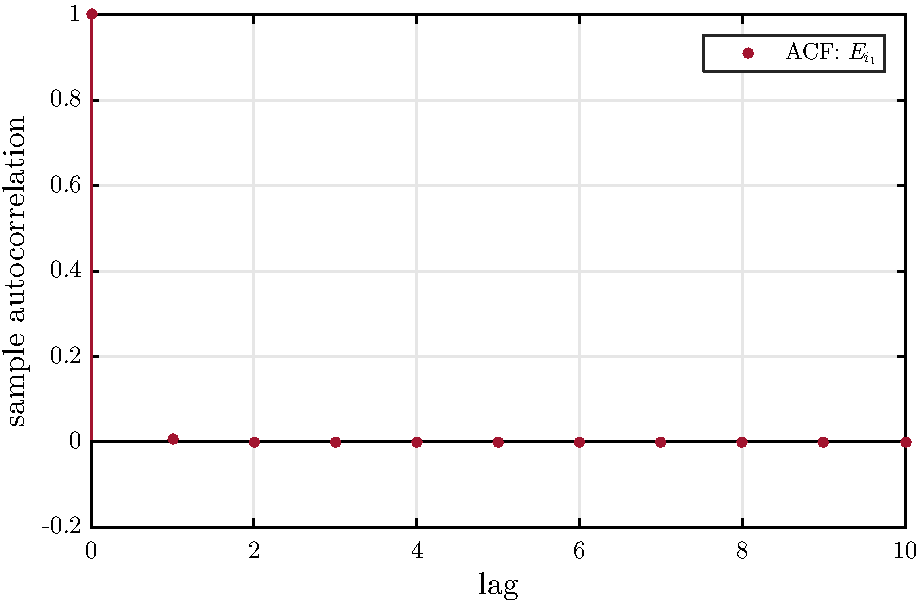
\includegraphics[width=\JRUESfigWidth]{fig_JRUES_ACF_HMC1}
    \caption[HMC: ACF of \(E_{i_1}\)]{HMC: ACF of \(E_{i_1}\).}
    \label{fig:ACF:HMC1}
  \end{minipage}%
  \hfill
  \begin{minipage}[b]{0.49\linewidth}
    \centering
    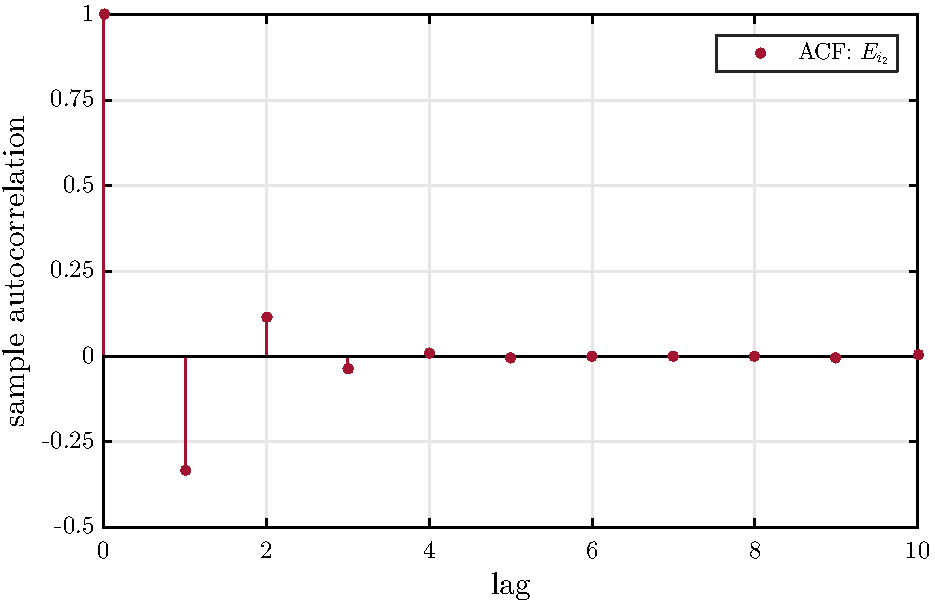
\includegraphics[width=\JRUESfigWidth]{fig_JRUES_ACF_HMC2}
    \caption[HMC: ACF of \(E_{i_2}\)]{HMC: ACF of \(E_{i_2}\).}
    \label{fig:ACF:HMC2}
  \end{minipage}%
\end{figure}
